% docs/texte/20_core/correlator.tex -- chapter "Correlator" (Interferosim)
% Version: 0.2.0 (2026-11-01) -- section "XF and FX" (interferosim 0.9.1)
%   0.1.0 (2026-10-31): FX correlator (interferosim 0.6.0)
% ================================================================
\label{ch:correlator}
\index{correlator}\index{FX correlator}\index{fringe search}

The correlator combines the independently recorded IQ streams of the
stations into visibilities. \texttt{interferosim.signal.FXCorrelator}
implements the FX scheme with the correlation kernels taken over from AAS6
\texttt{modules/interfero/correlate.py} 1.0.0 (\texttt{fractional\_delay},
\texttt{integer\_align}, \texttt{fringe\_stop}, \texttt{Accumulator},
\texttt{cross\_spectrum}, \texttt{delay\_rate\_search},
\texttt{apply\_fringe\_solution}, \texttt{stokes\_from\_products}; behaviour
unchanged). Notebook: \texttt{05\_correlator.ipynb}.

\section{Processing chain}

\begin{enumerate}
  \item \textbf{Model correction}: each station is shifted by the geometric
        delay $\tau_g(t)$ of the phase centre and multiplied by
        $e^{+2\pi i f_c\tau_g(t)}$ (delay tracking and fringe stopping,
        chapter~\ref{ch:signal}).
  \item \textbf{Fringe solution}: clock offsets (residual delay
        $\Delta\tau$) and LO offsets (residual rate $\Delta f$) are not in the
        model. \texttt{delay\_rate\_search} fringe-stops the station with a
        grid of trial rates and takes the delay from the peak of the lag
        spectrum; the maximum of the search surface is the solution.
        \texttt{refine\_fringe\_solution} (new in Interferosim) removes the
        sub-sample bias of the quadratic peak interpolation (up to about
        0.3 samples) by fitting the remaining phase slope across the band
        and the remaining phase drift over sub-segments.
  \item \textbf{F}: windows of $N_\mathrm{FFT}$ samples, Hann window, FFT;
        channel width $f_s/N_\mathrm{FFT}$.
  \item \textbf{X}: $X_i(f)\,X_j^*(f)$ averaged over the integration time,
        divided by the window power $\sum w^2$ -- the visibility per channel
        in Jy. Weight per channel from the auto spectra,
        $\sigma^2 = \langle|X_i|^2\rangle\langle|X_j|^2\rangle/(2n_\mathrm{win})$.
\end{enumerate}
The result is a \texttt{VisData} set with a frequency axis
(chapter~\ref{ch:data-formats}), one row per integration and baseline; the
header records $N_\mathrm{FFT}$, integration time, window, model correction
and the stations with a fringe solution.

\section{Signatures of the station errors}

A residual delay gives a phase slope across the band,
$\Delta\varphi(f) = -2\pi f\,\Delta\tau$, and shifts the peak of the lag
spectrum; a residual rate turns the phase in time, $2\pi\,\Delta f\,t$, and
smears the lag peak. Both make the channel-averaged visibility collapse
(Fig.~\ref{fig:fx-before}).

\begin{figure}[htbp]
  \centering
  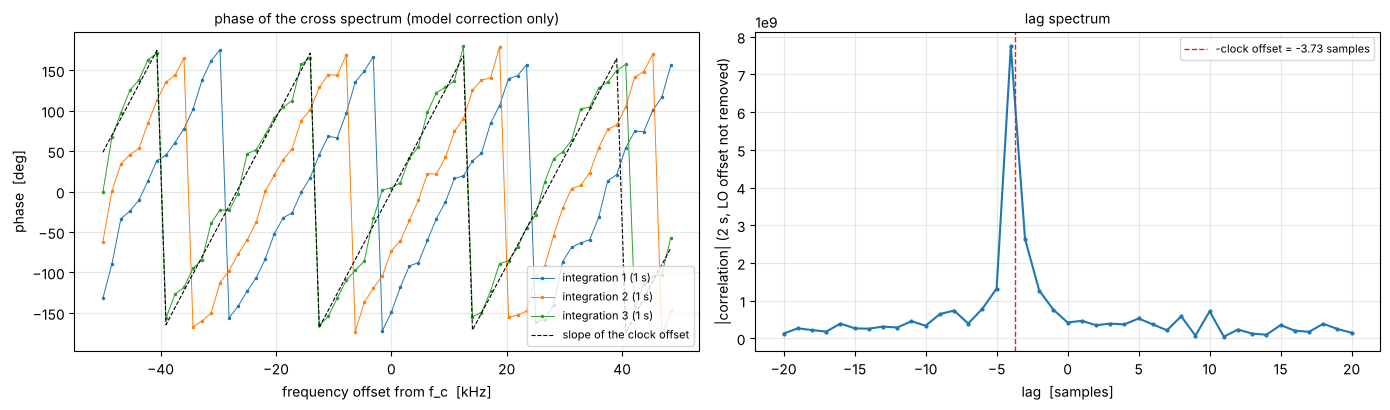
\includegraphics[width=\textwidth]{images/fx_before_solution.png}
  \caption{Sun with two 3\,m dishes 15\,m east--west, each with its own
           B210; station B with a clock offset of 37.3\,$\mu$s and an LO offset
           of 0.8\,Hz. Left: phase of the cross spectrum after the model
           correction (three 1-s integrations) with the slope of the clock
           offset; right: lag spectrum of 2\,s.}
  \label{fig:fx-before}
\end{figure}

\begin{figure}[htbp]
  \centering
  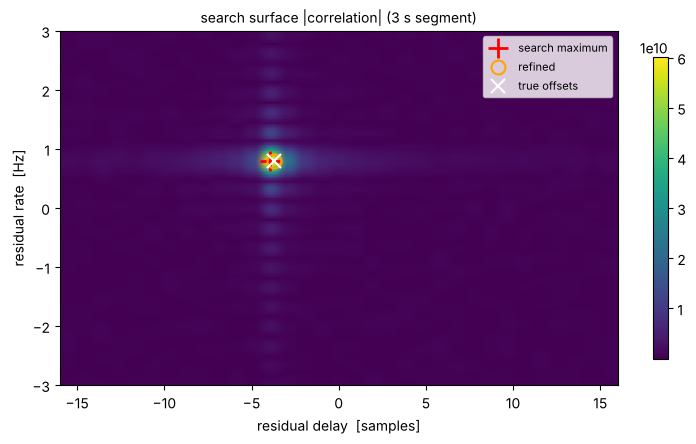
\includegraphics[width=0.75\textwidth]{images/fx_search_surface.png}
  \caption{Search surface of \texttt{delay\_rate\_search} (3\,s segment): search
           maximum, refined solution and the true offsets.}
  \label{fig:fx-search}
\end{figure}

\section{Result}

In the example of Fig.~\ref{fig:fx-before} the search finds
$-3.95$ samples and $+0.800$\,Hz; refined $-3.729$ samples ($-37.29\,\mu$s,
true $-37.30\,\mu$s) and $+0.801$\,Hz (Fig.~\ref{fig:fx-search}). After the
solution the phase is flat across the band and stable in time, the channel
averages agree with the model visibility (227\,kJy) to better than 1\,\%
(Fig.~\ref{fig:fx-after}). A constant phase offset may remain -- the LO phase
of each station is unknown and is calibrated on a calibrator source in a
real observation. The noise per channel grows with $\sqrt{N_\mathrm{FFT}}$,
the noise of the channel average does not depend on $N_\mathrm{FFT}$.

\begin{figure}[htbp]
  \centering
  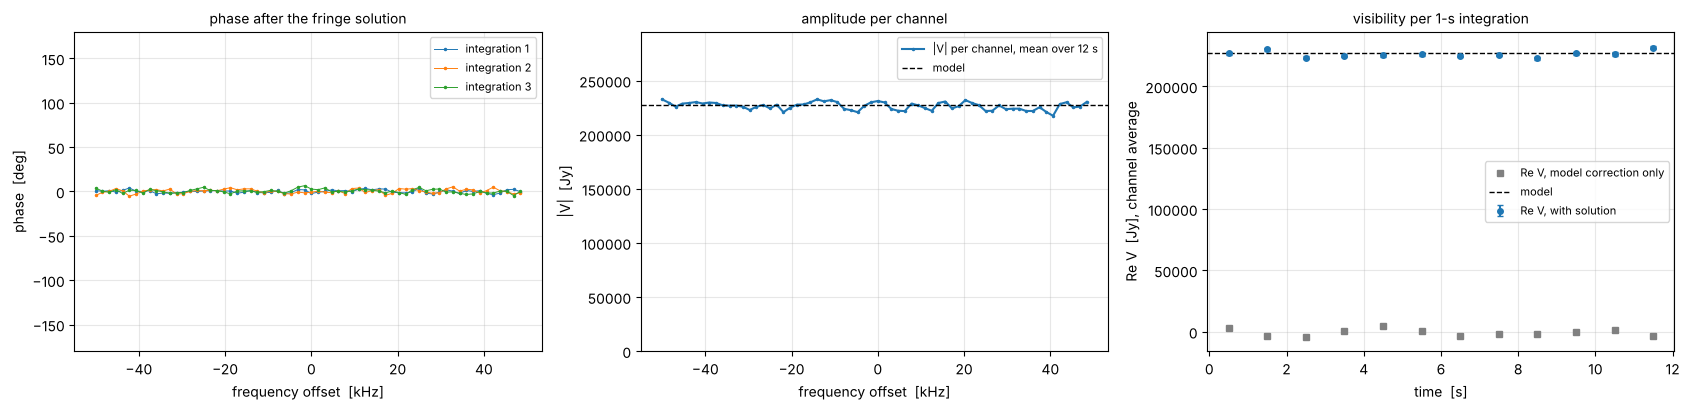
\includegraphics[width=\textwidth]{images/fx_after_solution.png}
  \caption{After the fringe solution: phase across the band, amplitude per
           channel (mean over 12\,s), channel-averaged visibility per 1-s
           integration with and without the solution.}
  \label{fig:fx-after}
\end{figure}

\section{XF and FX}
\label{sec:xf-fx}
\index{XF correlator}\index{Wiener--Khinchin theorem}\index{delay beam}

The cross-correlation function and the cross spectrum are a Fourier pair
(Wiener--Khinchin),
$R_{ab}(\tau) = \langle a(t+\tau)\,b^*(t)\rangle \leftrightarrow
S_{ab}(f) = \langle A(f)\,B^*(f)\rangle$. Version~0.9.1 adds the XF route for
comparison (theory notebook \texttt{B\_fourier.ipynb}):
\texttt{lag\_correlation} computes $R(k)$ over the lags $-N/2 \dots N/2-1$,
\texttt{xf\_cross\_spectrum} its Fourier transform in the channel layout and
unit of \texttt{Accumulator.visibility()/window\_power}.

For two noise streams with correlated power 1 and a delay of 3.4 samples
both correlators give the delay from the phase slope across the band (3.395
and 3.397 samples); the FX amplitude is lower by $(N-\tau)/N = 0.947$ for
$N = 64$, because a block of one station contains only $N-\tau$ samples of
the signal in the corresponding block of the other -- the reason why the FX
correlator removes the delay before the FFT (Fig.~\ref{fig:xf-fx}). Per sample
and baseline XF needs $N$ multiplications, FX about $\log_2 N + 1$ operations:
a factor 9 for 64 and 315 for 4096 channels.

A residual delay $\tau$ reduces the band-averaged amplitude by
$|\mathrm{sinc}(B\tau)|$, the Fourier transform of the flat band (delay beam);
first null at $1/B = 500$\,ns for the 2\,MHz of the B210, 10\,\% loss at
130\,ns (Fig.~\ref{fig:delay-beam}). The geometric delay of the 11.5\,km
baseline reaches 38\,\textmu s, 77 times $1/B$.

\begin{figure}[htbp]
  \centering
  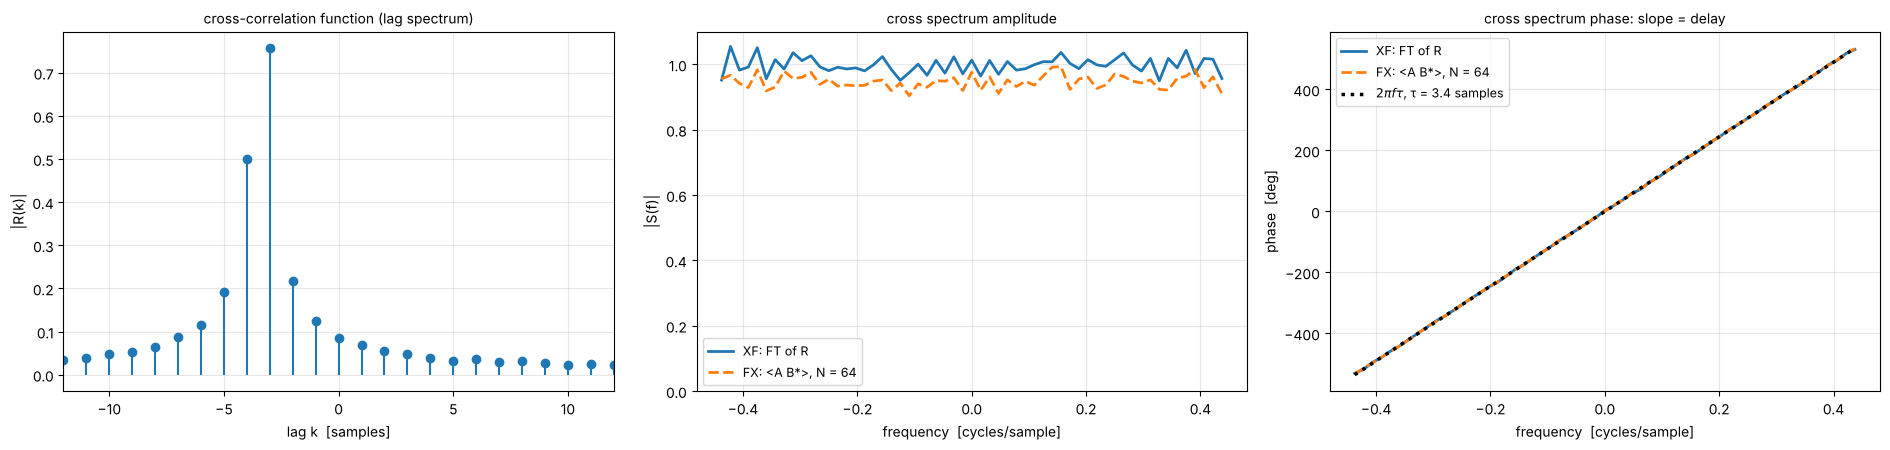
\includegraphics[width=\textwidth]{images/fourier_xf_fx.png}
  \caption{Lag spectrum, cross-spectrum amplitude and phase of the XF and the
           FX correlator for a delay of 3.4 samples.}
  \label{fig:xf-fx}
\end{figure}

\begin{figure}[htbp]
  \centering
  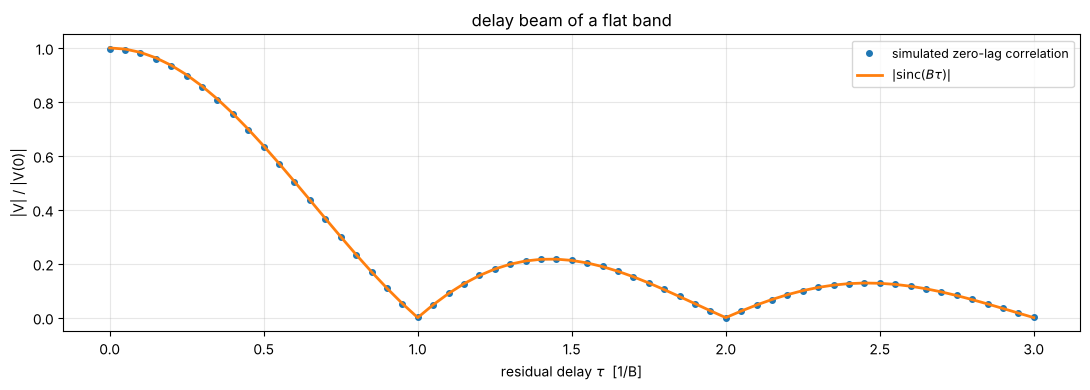
\includegraphics[width=0.75\textwidth]{images/fourier_delay_beam.png}
  \caption{Delay beam of a flat band: simulated zero-lag correlation against
           $|\mathrm{sinc}(B\tau)|$.}
  \label{fig:delay-beam}
\end{figure}
